
%-------------------------------------------------------------------------
\section{Jump Flooding-Cut}
\label{section jfcut}

\begin{figure*}
\centering
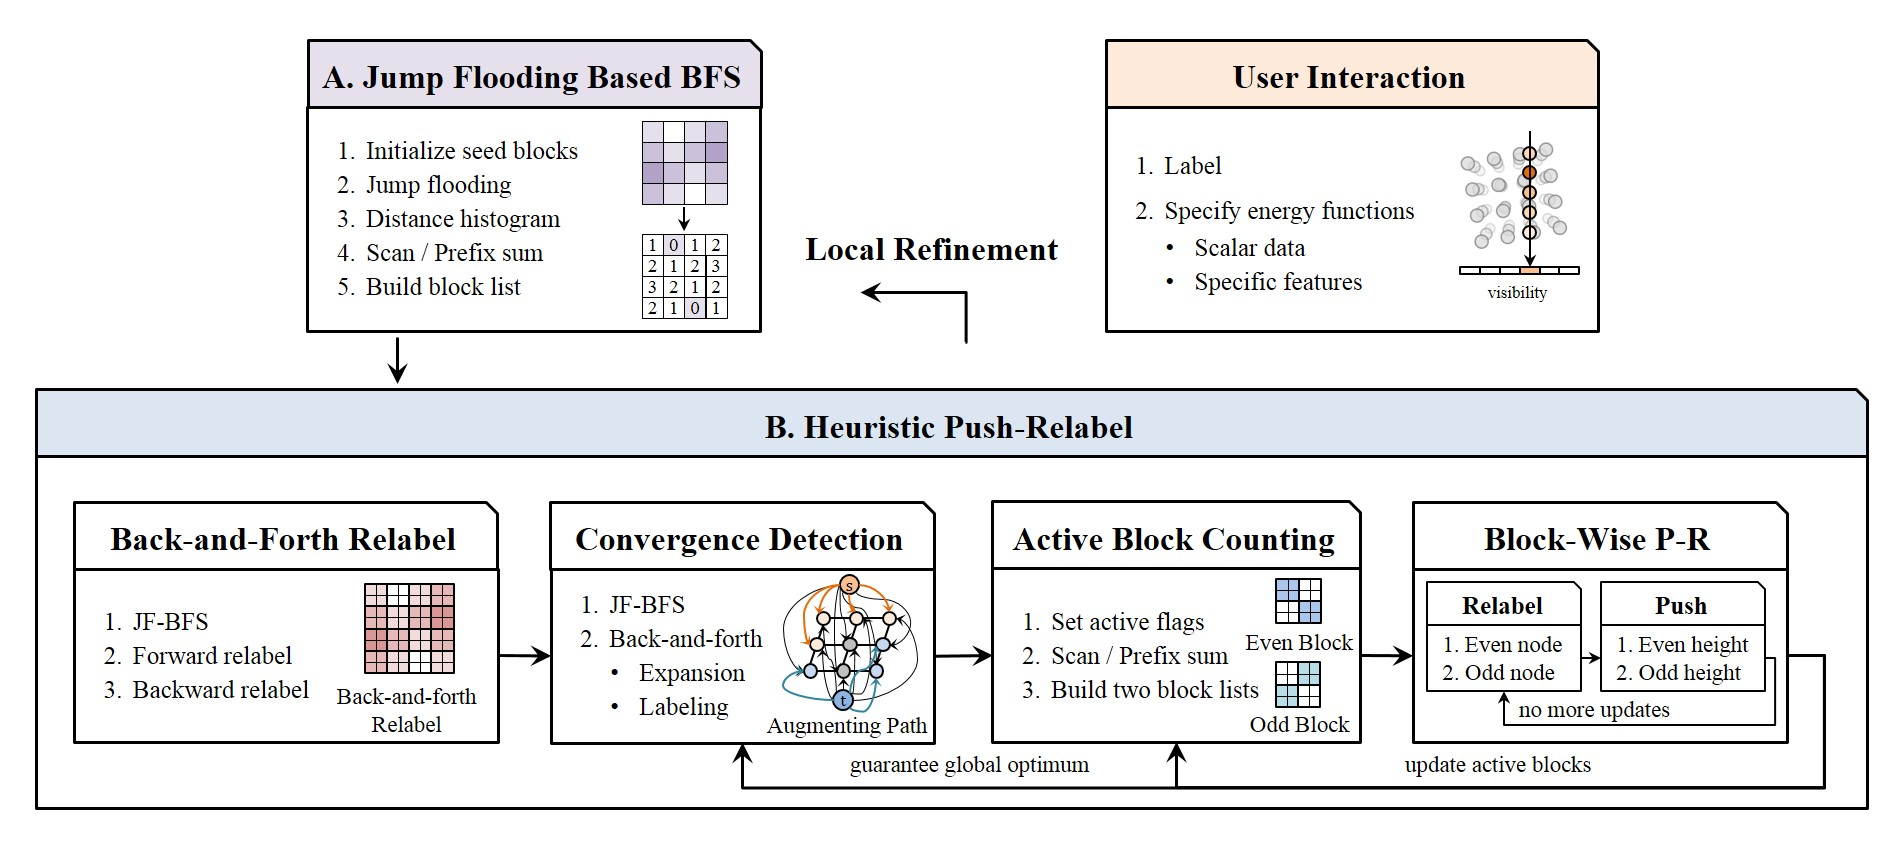
\includegraphics[width=17cm]{figures/fig1.jpg}
\caption{Our approach consists of two parts: jump flooding based BFS and heuristic push-relabel.
}
\label{figure overview}
\end{figure*}

%-------------------------------------------------------------------------
\subsection{Preliminary Knowledge}

\paragraph*{\textbf{Push-Relabel}}
starts with an excess flow (or preflow, allowing a node to have more outwards flow than inwards flow) and pushes an excess flow closer towards a sink (if the excess flow cannot reach a sink, it is pushed backwards to a source), until the maximum flow is found.
Because different active nodes (with excess flows) can be pushed or relabeled simultaneously, this algorithm has a high parallelism.
Moreover, several heuristic schemes, such as \textit{Global Relabel} and \textit{Gap Heuristics}, can be used to further improve the performance.

\paragraph*{\textbf{Global Relabel}}

computes height values (lower bound of the node's distance from the sink in the residual graph) by performing a Breadth-First Search (BFS) starting from the sink.
This heuristic technique can greatly reduce the number of iterations, because it implicitly finds out the augmenting-paths and pushes a node in the optimal direction.
This technique is used in the first stages of our approach because recomputing the height field (formed by the height of each node) in later stages is not effective and time-consuming.

\paragraph*{\textbf{Convergence Detection}}

starts from a source (or a sink) and performs a BFS on the residual network to check whether a path from a source to a sink exists:
no existence means the minimum cut is found, which partitions the graph into two parts; otherwise, the push-relabel should be continued.
Generally, the search should start from a source, because it allows us to do labeling at the same time, instead of starting from a sink and reversing its results to get the set of all neutral nodes (belonging to neither foreground, nor background) which is useless.
This technique ensures optimal results and avoids unnecessary iterations.

\paragraph*{\textbf{Jump Flooding}}

was first used to compute Voronoi Diagram (similar to Euclidean Distance Transform) for various applications in Computation Geometry and Pattern Recognition \cite{03MQR, 06RT}.
It can quickly compute the \textit{Nearest Seed Point} (NSP) of each point.
The main idea is to replace the NSP of the current point with the nearest one of the NSPs of all its neighboring points. The size of the neighborhood is halved in each iteration.
\textit{Jump Flooding} (JF) can be used to accelerate BFS in computing the nearest distance.
Given the nearest point, the nearest distance can be derived, if each neighboring point is connected with each other.
Section 3.2 gives an example of using JF to accelerate BFS.

%-------------------------------------------------------------------------
\subsection{Overview}

The key idea of our method is to accelerate the propagation of flow in the graph. We propose a convergence detection technique to ensure accuracy that is not achieved in \cite{08VN} and a block-wise push-relabel technique to achieve a faster convergence speed compared with \cite{11W}.

Our approach consists of two parts as shown in \figurename \ref{figure overview}: jump flooding based BFS and heuristic push-relabel.

Part A (jump flooding based BFS) is a basic module of our algorithm, which improves the performance of multi-pass global relabel and convergence detection.

Part B (heuristic push-relabel) is the core algorithm of our approach.
This part computes the maximum flow in an efficient way especially for large data sets, detailed in Section 3.4.
All these algorithms are parallelized with OpenCL (Open Computing Language), and evaluated with a variety of data sets.

We also design an intuitive user interface to help users specify foreground and background elements based on visibility, described in Section 4.
If the users are not satisfied with the results, they can do local refinement.

%-------------------------------------------------------------------------
\subsection{Jump Flooding Based BFS}

We use JF to accelerate Global Relabel and Convergence Detection, because both of them on the BFS.
In general, for GPU computing, the data set is often divided into blocks (each block can contain 64 to 512 threads) to fit the hardware architecture for high efficiency.
When the data set is small, using the CPU to fulfill BFS is adequate. However, when the size becomes much larger, the increasing cost should receive additional consideration.
For instance, if the data size is $1024 \times 1024 \times 512$ and the maximum block size is 256, we have to deal with nearly four million blocks.
Accordingly, we introduce a Jump Flooding based algorithm (JF-BFS), which includes five steps:

{
\small
\begin{enumerate}
\item[\textbf{F1}] Initialize all the seed blocks that contain seed nodes;
\item[\textbf{F2}] Perform jump flooding;
\item[\textbf{F3}] For each block, compute its nearest distance to the seed blocks and the distance histogram;
\item[\textbf{F4}] Perform the scan primitive on the distance histogram;
\item[\textbf{F5}] Build the block list according to the prefix sum of distance histogram.
\end{enumerate}
}

Note that, all the above steps can be performed on the GPU.
In \textbf{F1}, a seed block is defined to have at least one foreground or background node, whose \textit{Nearest Seed Block} (NSB) is initialized as itself.
Other blocks' NSBs are set to infinity.
In \textbf{F2}, we perform the standard Jump Flooding Algorithm (JFA).
In \textbf{F3}, for each block $\mathbf{p}$, we compute the distance to its NSB as the nearest distance $h$ to all the seed blocks (see Algorithm 1).
In \textbf{F4}, we compute the distance histogram and label each block a corresponding order in the bin.
In \textbf{F5}, we compute its prefix sum \cite{11MG} and calculate the final positions of all the blocks in the list.

\begin{figure}
\centering
\subfigure[Jump Size $2$]{
    \label{figure step 2}
    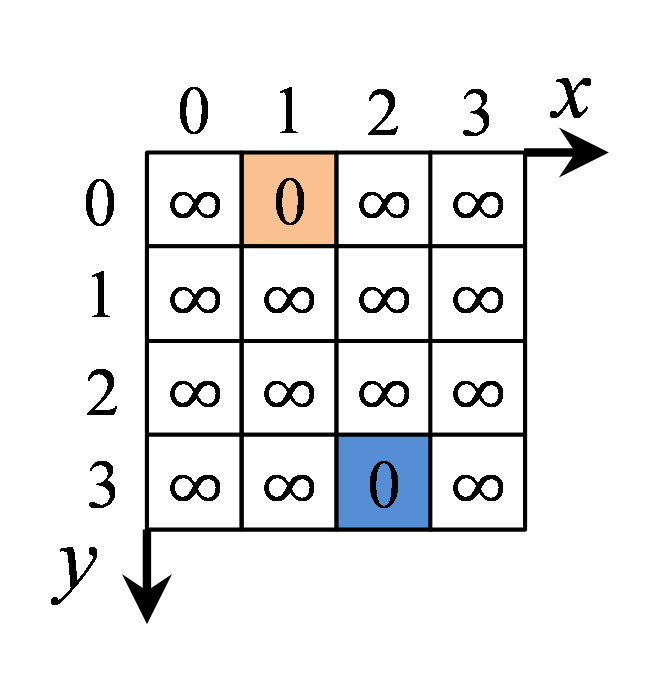
\includegraphics[width=2.55cm]{figures/fig3a.png}
    }
\subfigure[Direction $X$]{
    \label{figure step 2 x}
    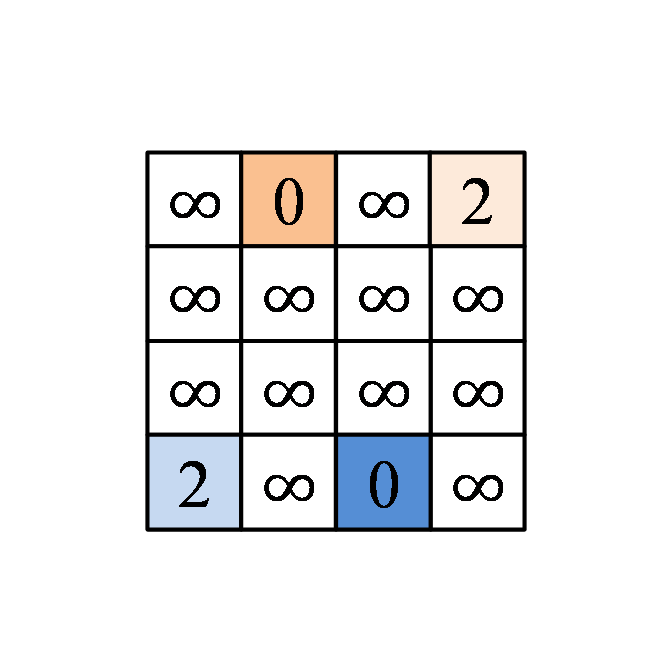
\includegraphics[width=2.55cm]{figures/fig3b.png}
    }
\subfigure[Direction $Y$]{
    \label{figure step 2 y}
    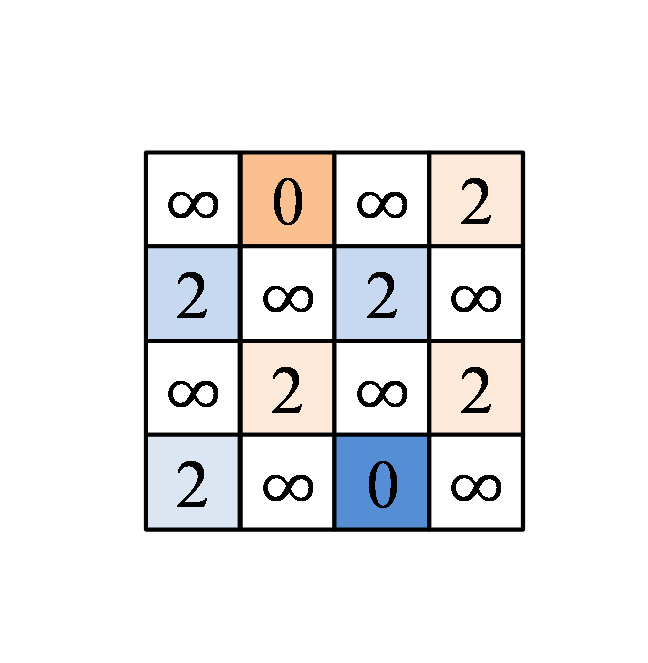
\includegraphics[width=2.55cm]{figures/fig3c.png}
    }
\\
\subfigure[Jump Size $1$]{
    \label{figure step 1}
    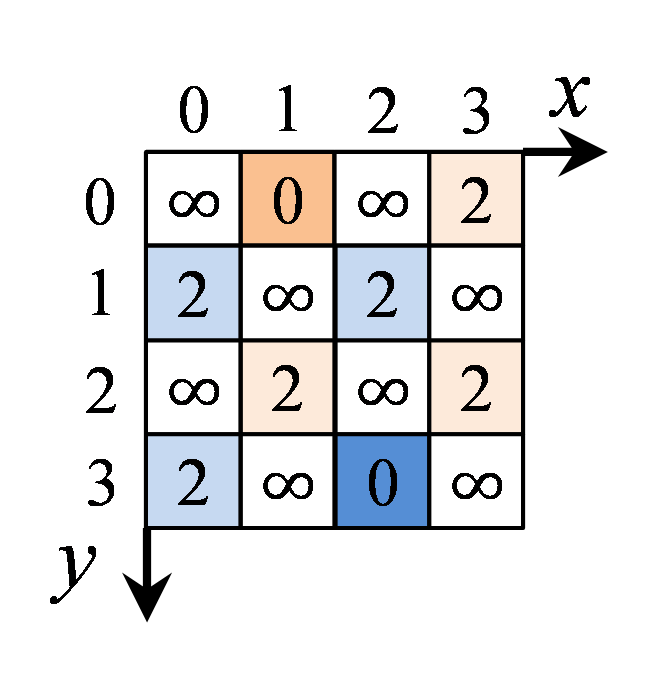
\includegraphics[width=2.55cm]{figures/fig3d.png}
    }
\subfigure[Direction $X$]{
    \label{figure step 1 x}
    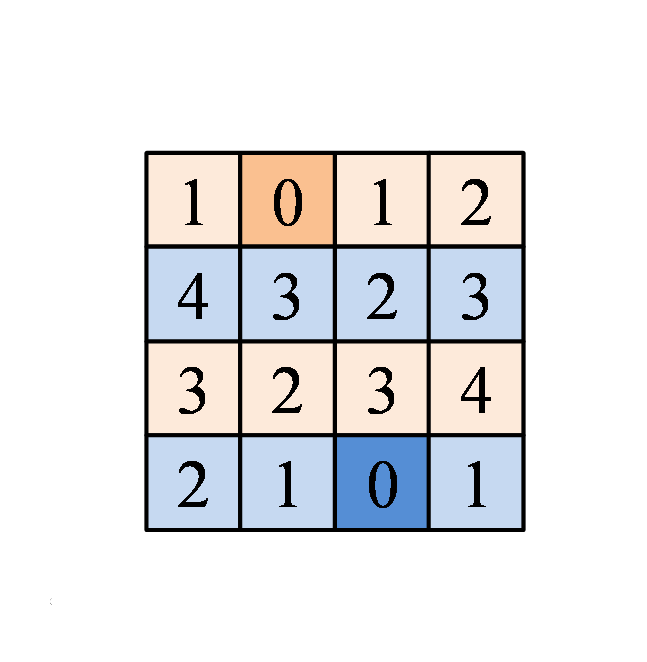
\includegraphics[width=2.55cm]{figures/fig3e.png}
    }
\subfigure[Direction $Y$]{
    \label{figure step 1 y}
    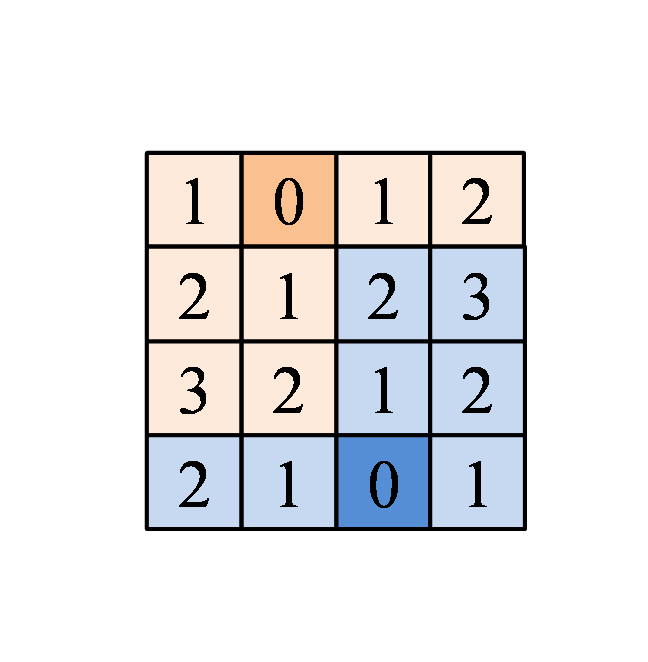
\includegraphics[width=2.55cm]{figures/fig3f.png}
    }
\caption{Jump Flooding. Two seed blocks are colored in dark orange and dark blue.
(a)-(c): the 1st flooding with $Size = 2$. Six blocks with light colors update their nearest seed blocks. Two of them are in $x$ direction and four of them are in $y$ direction.
(d)-(f): the 2nd flooding with $Size = 1$. The rest of the blocks updates the distances to their nearest seed blocks (see the integers in pixels).
}
\label{figure jump flooding}
\end{figure}

\figurename \ref{figure jump flooding} illustrates the process by taking a $4 \times 4$ network as an example.
The seed blocks are (1,0) and (2,3) and the number inside a block shows the current distance to the NSB.
In this case, the JFA includes two iterations.
The step size in the first iteration is 2 (\figurename \ref{figure step 2}-\ref{figure step 2 y}) while in the second iteration it is halved to be 1 (\figurename \ref{figure step 1}-\ref{figure step 1 y}).
In the first iteration, according to the neighbors in the $x$ direction, the NSBs of block (3, 0) and (0, 3) are updated to (1, 0) and (0, 3) respectively.
After that, block (0, 1), (2, 1), (0, 3) and (2, 3) are updated by taking the vertical neighbors into consideration.
In the second iteration, we process these blocks in the same way using a smaller step size.
Finally, eight blocks, colored in yellow have the same NSB - block (1, 0) while the other blocks, colored in blue are the nearest to block (2, 3), see \figurename \ref{figure step 1 y}.
The corresponding pseudo code is:

\begin{algorithm}
\label{algorithm jump flooding}
\caption{$\texttt{Jump Flooding}(Size, Nearest)$}
\begin{algorithmic}
\STATE $\mathbf{p} \leftarrow \texttt{Global-ID}$
\STATE $\mathbf{q} \leftarrow Nearest[x_p, y_p]$
\STATE $d \leftarrow \texttt{Taxicab-Distance} (\mathbf{p}, \mathbf{q})$
\FOR {each $\mathbf{p}_t \in \texttt{Neighbors} (\mathbf{p}, Size)$}
    \STATE $\mathbf{q}_t \leftarrow Nearest[x_{p_t}, y_{p_t}]$
    \STATE $d_t \leftarrow \texttt{Taxicab-Distance} (\mathbf{p}, \mathbf{q}_t)$
    \IF{$d_t < d$}
        \STATE $d \leftarrow d_t$
        \STATE $\mathbf{q} \leftarrow \mathbf{q}_t$
    \ENDIF
\ENDFOR
\STATE $Nearest[x_p, y_p] \leftarrow \mathbf{q}$
\end{algorithmic}
\end{algorithm}

%-------------------------------------------------------------------------
\subsection{Heuristic Push-Relabel}
\label{section hpr}

The basic idea of \textit{Heuristic Push-Relabel} is to process a block like a node, meaning that the push and relabel operations are repeated inside a block until it is saturated (no more updates for push and relabel).
Compared to the global push or relabel scheme, ours has two advantages.
First, the synchronization operations in a block can avoid data conflict for push and relabel, and local memory can be efficiently used to cache intermediate data.
Second, an alternate push and relabel improves the propagation speed of information because a node along each direction is pushed at the same time.

This scheme is more efficient than \textit{Wave Push} which only handles one direction each time.
Moreover, it allows us to take advantage of data locality and skip some of the directions.

Our method includes 4 steps:

{
\small
\begin{enumerate}
\item[\textbf{H1}] Perform JF-BFS to build the block list and perform a back-and-forth relabel;
\item[\textbf{H2}] Repeat \textbf{H3} $k_1$ times and use JF-BFS to build the list and perform the convergence detection;
    \begin{enumerate}
    \item[\textbf{H2.1}] Perform JF-BFS to build the block list starting from the foreground nodes and repeat \textbf{H2.2} until detection failed or no more nodes are marked;
    \item[\textbf{H2.2}] Perform back-and-forth detection;
        \begin{enumerate}
        \item[\textbf{H2.2.1}] If any background node is found return to \textbf{H2.1} (detection fails, keep iterating), otherwise repeat \textbf{H2.1.2} until no more nodes are marked (detection succeeds, stop iterating);
        \item[\textbf{H2.2.2}] Mark the current node as visited according to the state (visited or not) of its neighbors.
        \end{enumerate}
    \end{enumerate}
\item[\textbf{H3}] Repeat \textbf{H4} $k_2$ times, count active blocks and use Scan to build two block lists for even blocks and odd blocks;
    \begin{enumerate}
    \item[\textbf{H3.1}] For each block, set its flag as whether it contains active nodes;
    \item[\textbf{H3.2}] Perform scan primitive on the flags;
    \item[\textbf{H3.3}] Build two lists for even and odd blocks respectively;
    \end{enumerate}
\item[\textbf{H4}] Perform push-relabel for even blocks and odd blocks respectively;
    \begin{enumerate}
    \item[\textbf{H4.1}] Repeat \textbf{H4.1} until no more nodes can be pushed;
    \item[\textbf{H4.2}] Relabel even nodes and odd nodes respectively, then push them in the same way.
    \end{enumerate}
\end{enumerate}
}

%-------------------------------------------------------------------------
\subsubsection{Back-and-Forth Relabel}

In \textbf{H1}, we first use JF-BFS to build the block list for subsequent scheduling.
Based on the list, we perform a back-and-forth relabel, which processes the blocks in an ascending order and then in a descending order.
It can help us find out the paths that often change directions.
The reason is that after we finish relabel in one direction, the paths that pass along the same direction have already been found and we can easily find out all paths that change their directions only once if we try an opposite direction.
For JF-BFS, the seed blocks include background nodes (with negative excess flow).

%-------------------------------------------------------------------------
\subsubsection{Convergence Detection}

In \textbf{H2}, we detect global convergence while labeling the cutting results by checking whether there exists an augmenting-path in the residual network.
If so, we need further actions to increase the flow, otherwise we found the maximum flow.
We perform JF-BFS from the foreground nodes (source-connected) because it can mark the final results and avoid neutral nodes (see Section 3.1).

The principle implied by these sub-steps is that when we get the maximum flow(or minimum cut), the residual network will be divided into two parts, and for each part all nodes should be connected, and all edges belonging to the minimum cut should be saturated.
It indicates that we can start from one part and repeat expanding nodes to decide whether we have found the global optimum.

This step ensures that our algorithm can find the maximum flow and get the optimal results.
In our implementation, due to the expensive cost of this procedure, we repeat \textbf{H3} $k_1$ times and perform it once.
$k_1$ defaults to 4 (performs best for median-size image) and can be specified by users.
Generally, it would be better to increase $k_1$ when the data size increases (16 is better for large images and videos).

%-------------------------------------------------------------------------
\subsubsection{Active Block Counting}

Active Block Counting is designed to reduce the computational cost by building a block list for active blocks, which is mainly based on the two facts: during the process only some nodes can be pushed or relabeled, and the number of active nodes decreases when more data is processed.
So only process active nodes efficiently improve the performance.
Because active-blocks change slowly, we can do one counting after $k_2$ iterations.
$k_2$ is set to be 4 (better for median-size data sets) and is user-adjustable.
This procedure includes three sub-steps (see \textbf{H3.1}~\textbf{H3.3}).
We use two flags to record the detection results.
If the current block contains active nodes, we set its corresponding flag (even flag corresponds to even block) to be 1, otherwise 0.
After that, we perform a scan to compact the flags into a scheduling list.

%-------------------------------------------------------------------------
\subsubsection{Block-Wise Push-Relabel}

\begin{figure}
\centering
\subfigure[Wave Push]{
    \label{figure wave push}
    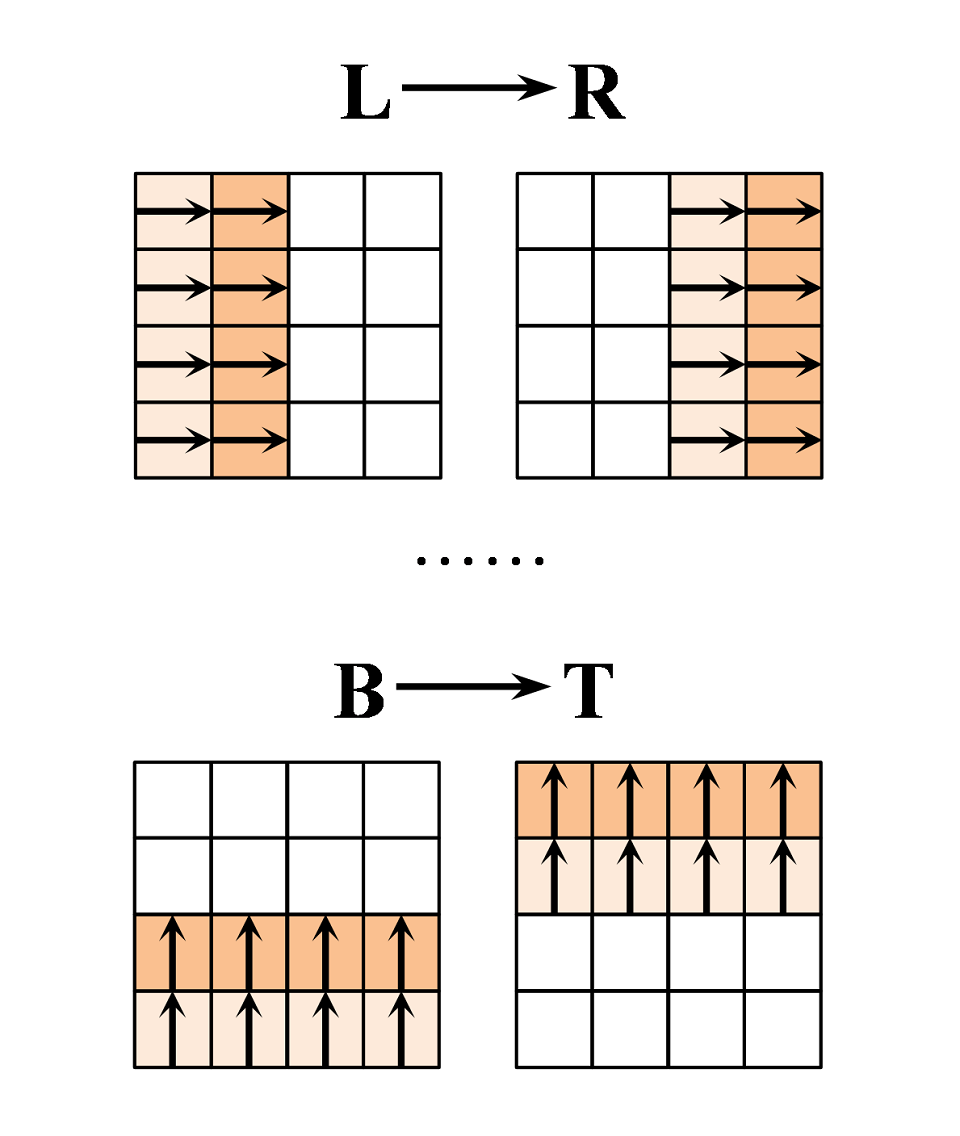
\includegraphics[width=3.5cm]{figures/fig4a.png}
    }
\subfigure[Block-Wise Push]{
    \label{figure block-wise push}
    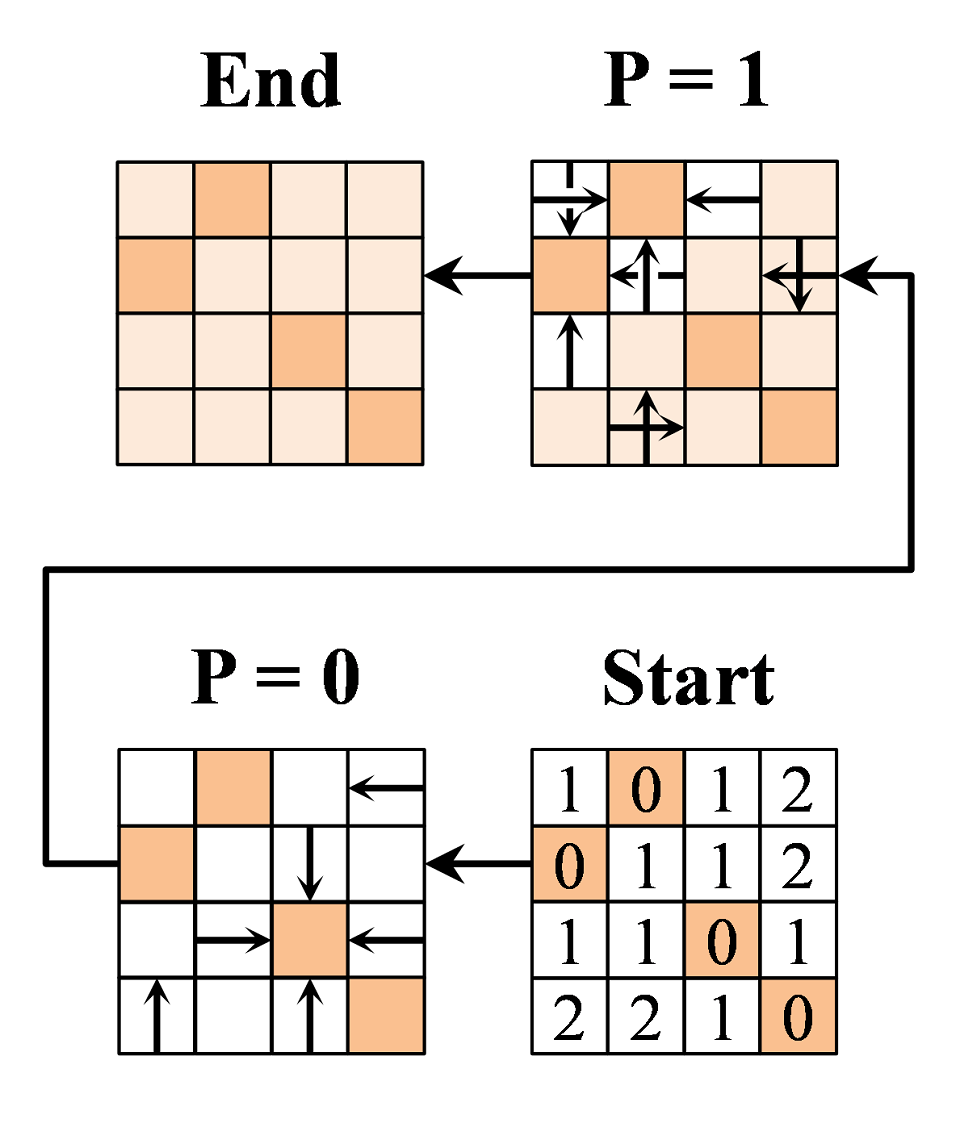
\includegraphics[width=3.5cm]{figures/fig4b.png}
    }
\caption{Heuristic Push.
(a): only handles one direction each time.
(b): skip some directions which needn't to be processed. $P$ denotes block parity.
}
\label{figure heuristic push}
\end{figure}

As mentioned earlier, iterative push-relabel operations inside a block takes advantage of locality and increases the propagation speed of flow compared with \textit{Wave Push} as shown in \figurename \ref{figure heuristic push}.

\begin{algorithm}
\label{algorithm block-wise p-r}
\caption{$\texttt{Push-Relabel}(Node)$}
\begin{algorithmic}
\STATE $\mathbf{p} \leftarrow \texttt{Local-ID}$
\STATE copy global $Node$ to local $Node'$
\STATE $d' \leftarrow false$
\STATE \texttt{barrier()}
\WHILE {\NOT $d'$}
    \STATE $t_a \leftarrow \texttt{Active}(Node'[x_p, y_p])$
    \STATE $t_p \leftarrow (x_p + y_p)$ mod $2$
    \IF{$t_a$ \AND $t_p = 0$}
       \STATE $ \texttt{Relabel}()$
    \ENDIF
    \STATE \texttt{barrier()}
    \IF{$t_a$ \AND $t_p = 1$}
       \STATE $ \texttt{Relabel}()$
    \ENDIF
    \STATE $d' \leftarrow true$
    \STATE \texttt{barrier()}

    \STATE $t_a \leftarrow \texttt{Active}(Node'[x_p, y_p])$
    \IF{$t_a$ \AND $t_p = 0$ \AND $\texttt{Push}()$}
        \STATE $d' \leftarrow false$
    \ENDIF
    \STATE \texttt{barrier()}
    \IF{$t_a$ \AND $t_p = 1$ \AND $\texttt{Push}()$}
        \STATE $d' \leftarrow false$
    \ENDIF
    \STATE \texttt{barrier()}
\ENDWHILE
\STATE copy local $Node'$ to global $Node$
\end{algorithmic}
\end{algorithm}

The kernel code (2D-version) is shown in Algorithm 2.
We first load the data from global memory to local memory, then perform iterative push-relabel, and finally write back the data.
In each iteration, there are two stages: relabel and push.
In the relabel stage, we first check whether $Node'[x_p, y_p]$ is active, and then process even nodes with $(x_p + y_p) \, mod \, 2 = 0$ and odd nodes with $(x_p + y_p) \, mod \, 2 = 1$ respectively, because these two kinds of nodes have data conflict with each other.
In the push stage, we process the nodes in the same way.
Both directions are handled one after another.
When a node becomes inactive after being pushed in one direction, we skip the following directions.
In this way, many unnecessary computations can be avoided.
Then we process the nodes in the same way.
